\chapter{Indicadores Sociais}
\par Para identificar os níveis de pobreza de uma população, é primordial a classificação de aspectos para um padrão de vida digno e satisfatório, como dieta balanceada, vestimentas adequadas, acesso a serviços de saúde e educação, ambiente sadio, etc.
\begin{figure}[!h]
	\begin{subfigure}{\linewidth}
		\caption{Taxa de pobreza}
		\subcap{Linha de US\$5,50 PPC}
		\label{fig:pob}
		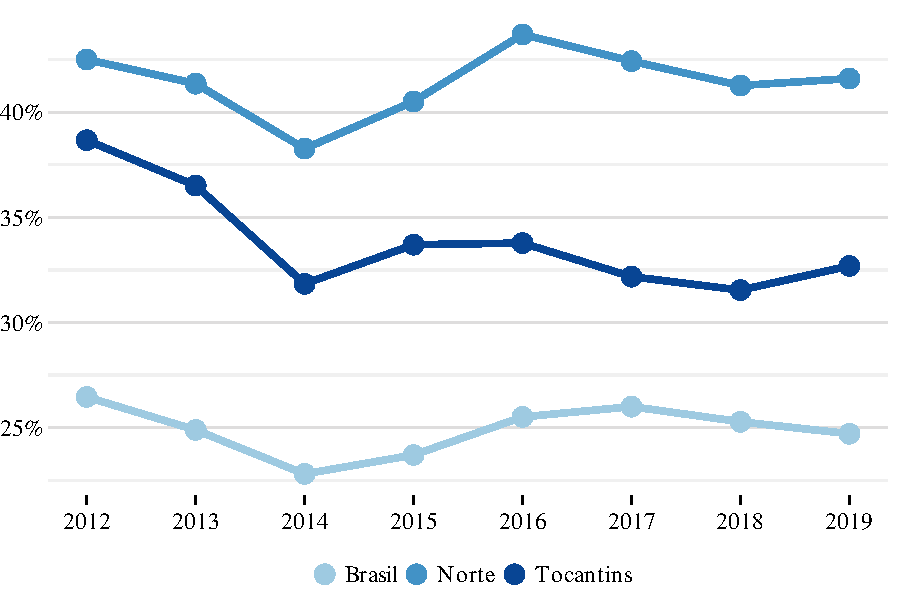
\includegraphics{fig/taxa_pobreza.pdf}
		\source{\acrshort{ibge}}
	\end{subfigure}
	\begin{subfigure}{\linewidth}
		\caption{Taxa de extrema pobreza}
		\label{fig:expob}
		\subcap{Linha de US\$1,90 PPC}
		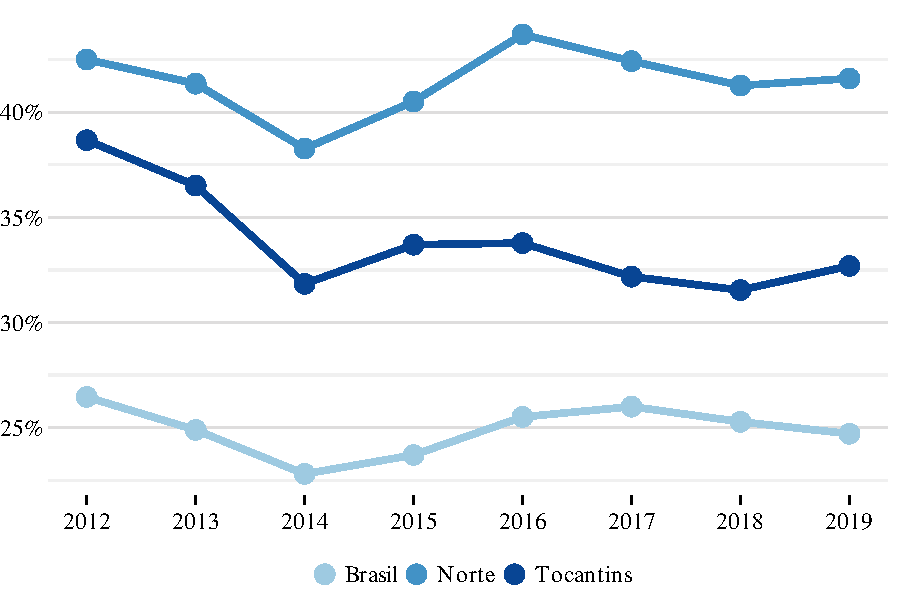
\includegraphics{fig/taxa_pobreza.pdf}
		\source{\acrshort{ibge}}
	\end{subfigure}
	\begin{subfigure}{\linewidth}
		\caption{Índice de Gini}
		\label{fig:gini}
		\subcap{Coeficiente de desigualdade}
		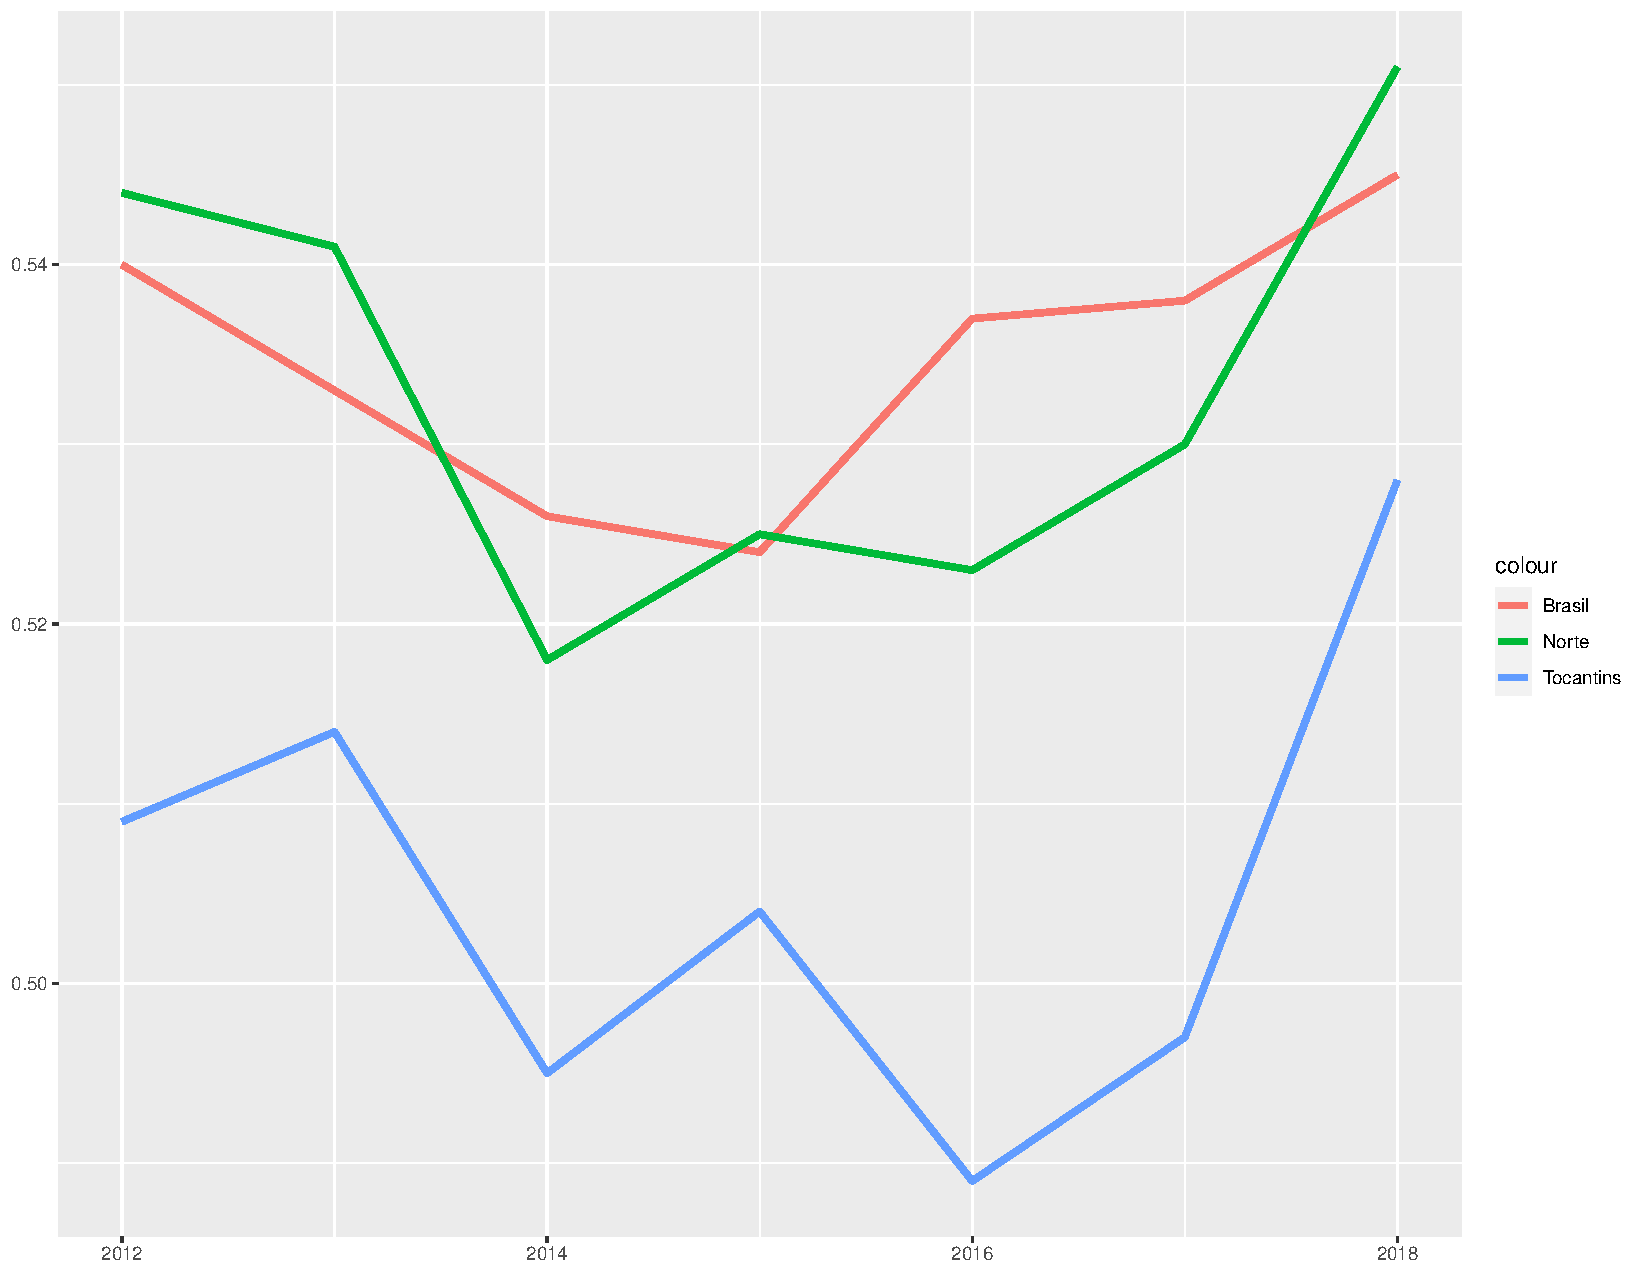
\includegraphics{fig/gini.pdf}
		\source{\acrshort{ibge}}
	\end{subfigure}
\end{figure}
%\par No Brasil, a Constituição Federal do Brasil de 1988, garante no Art. 6º que todos têm direitos sociais, estabelecendo dimensões para o bem-estar da população, como a educação, a saúde, a alimentação, o trabalho, a moradia, o transporte, o lazer, a segurança, a previdência social, a proteção à maternidade e à infância e a assistência aos desamparados.
\par Nesse sentido, cabe a pergunta: Como andam os indicadores sociais tocantinenses levando em conta os últimos anos foram marcados por um baixo crescimento econômico e pioras no mercado de trabalho? É possível ver na Figura \ref{fig:pob} a evolução da taxa de pobreza do estado entre 2012 e 2019, comparando com o desempenho da região Norte e com o Brasil.
\par Apesar do contexto, a taxa de pobreza do Tocantins apresentou uma queda de 38,67\% para 32,69\%, o que em números absolutos representou uma saída de cerca de 45 mil pessoas dessa condição. Uma queda expressiva, ainda mais se comparada o valor para a região Norte, que permaneceu praticamente estável durante o período, levando a um aumento da diferença em relação ao Tocantins. Já se comparada à taxa brasileira, a taxa tocantinense ainda é maior, porém houve uma diminuição dessa diferença, uma vez que a taxa nacional não apresentou grandes quedas nos anos analisados. Cabe porém um destaque com relação aos dados relacionados ao ano de 2019. Neste ano, mesmo com uma queda da taxa brasileira de 25,28\% para 24,71\%, no estado do Tocantins houve um aumento da taxa saindo de 31,54\% para 32,69\%.

\par Por outro lado, olhando com uma linha de pobreza menor, a dos extremamente pobres, os resultados não seguiram a mesma tendência, indicando um maior impacto do cenário apresentado para essa faixa. Os resultados são apresentados na Figura \ref{fig:expob}.

\par A taxa de extrema pobreza apresentou alta entre 2012 e 2019 no estado, saindo de 5,59\% para 7,98\%. Em termos absolutos de pessoas vivendo nessa condição, tem-se a mínima em 2014 onde a partir daí ocorre uma alta de 64,35\%, um detalhe que em muitas vezes pode passar desapercebido olhando somente para a taxa que neste período saiu de 5,14\% para 7,98\%. O mesmo comportamento pode ser observado no indicador para o Brasil e  com mais intensidade ainda para região Norte.

\par Sobre desigualdade de renda possível perceber que houve uma leve alta do índice de Gini no estado ao longo dos anos apresentados, saindo de 0,509 para 0,530, como pode ser visto na Figura \ref{fig:gini}. Essa alta vem seguindo a tendência dos outros indicadores apresentados até então. Para o Brasil e para região Norte, idem.
%\begin{smbox}[label={labelbox},nameref={tx_pobre_gini}]{Taxa de pobreza e índice de Gini}
%	É um índice que demonstra o grau de concentração de renda de um determinado grupo. Seus resultados variam entre 0 e 1. Quanto mais próximo de 0, mais igual é aquele grupo, e quanto mais próximo de 1, mas desigual é aquele grupo.
%	Uma das formas mais comuns de se mensurar pobreza é através de uma linha de pobreza absoluta, que define como pobres aqueles que vivem com uma renda inferior ao valor adotado pela linha. Neste sentido, o Banco Mundial sugere linhas que se adaptam melhor para as condições de vida de determinados países. Para um país de rendimento médio-alto, é sugerido uma linha de US\$5,50 \acrshort{ppc}.
%\end{smbox}
\par Os resultados apresentados nessa seção são produto, como já mencionado, do baixo crescimento econômico dos últimos anos e as suas consequências no mercado de trabalho, com aumento da taxa de desemprego, precarização dos trabalhos e aumento do trabalho informal. A crise fiscal enfrentada pela União e pelo estado do Tocantins de certa forma também contribui para esse quadro, uma vez que gastos com serviços básicos para a população são muitas vezes limitados nesse tipo de contexto, perpetuando o cenário apresentado.


